\chapter{Repeatability of Ambient Stability Experiments}\label{ch:appendixB}

\begin{figure}[htbp]
    \centering
    % Second row
    \begin{subfigure}[t]{0.5\textwidth}
        \centering
        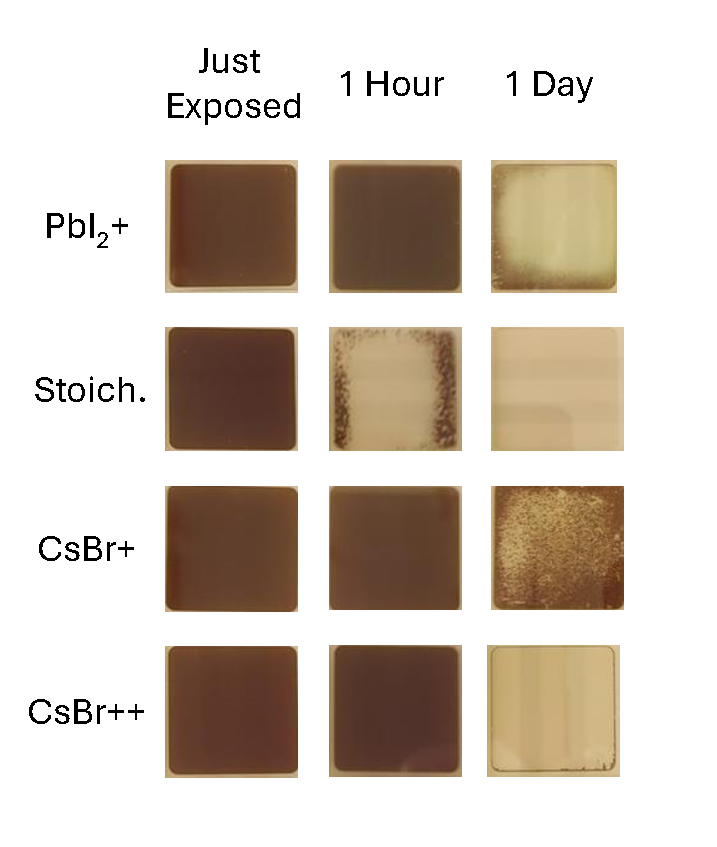
\includegraphics[width=\textwidth]{chapters/appendixB/images/Stability_Rotation_Stoichiometries_v2.pdf} % Replace with your image file
             
    \end{subfigure}

    \caption[Assessment of the ambient stability repeatability of \ch{CsPbI_2Br} thin films prepared with various nominal CsBr:\ch{PbI_2} molar ratios.]{Assessment of the ambient stability repeatability of \ch{CsPbI_2Br} thin films prepared with various nominal CsBr:\ch{PbI_2} molar ratios. These are second samples from the same deposition batches used for the stability measurements shown in Figure~\ref{fig:stability:stoichiomtries_rotation}a.}
    \label{fig:appendix:stoichiometry_rotation_V2}
\end{figure}


\begin{figure}[htbp]
    \centering
    % Second row
    \begin{subfigure}[t]{0.99\textwidth}
        \centering
        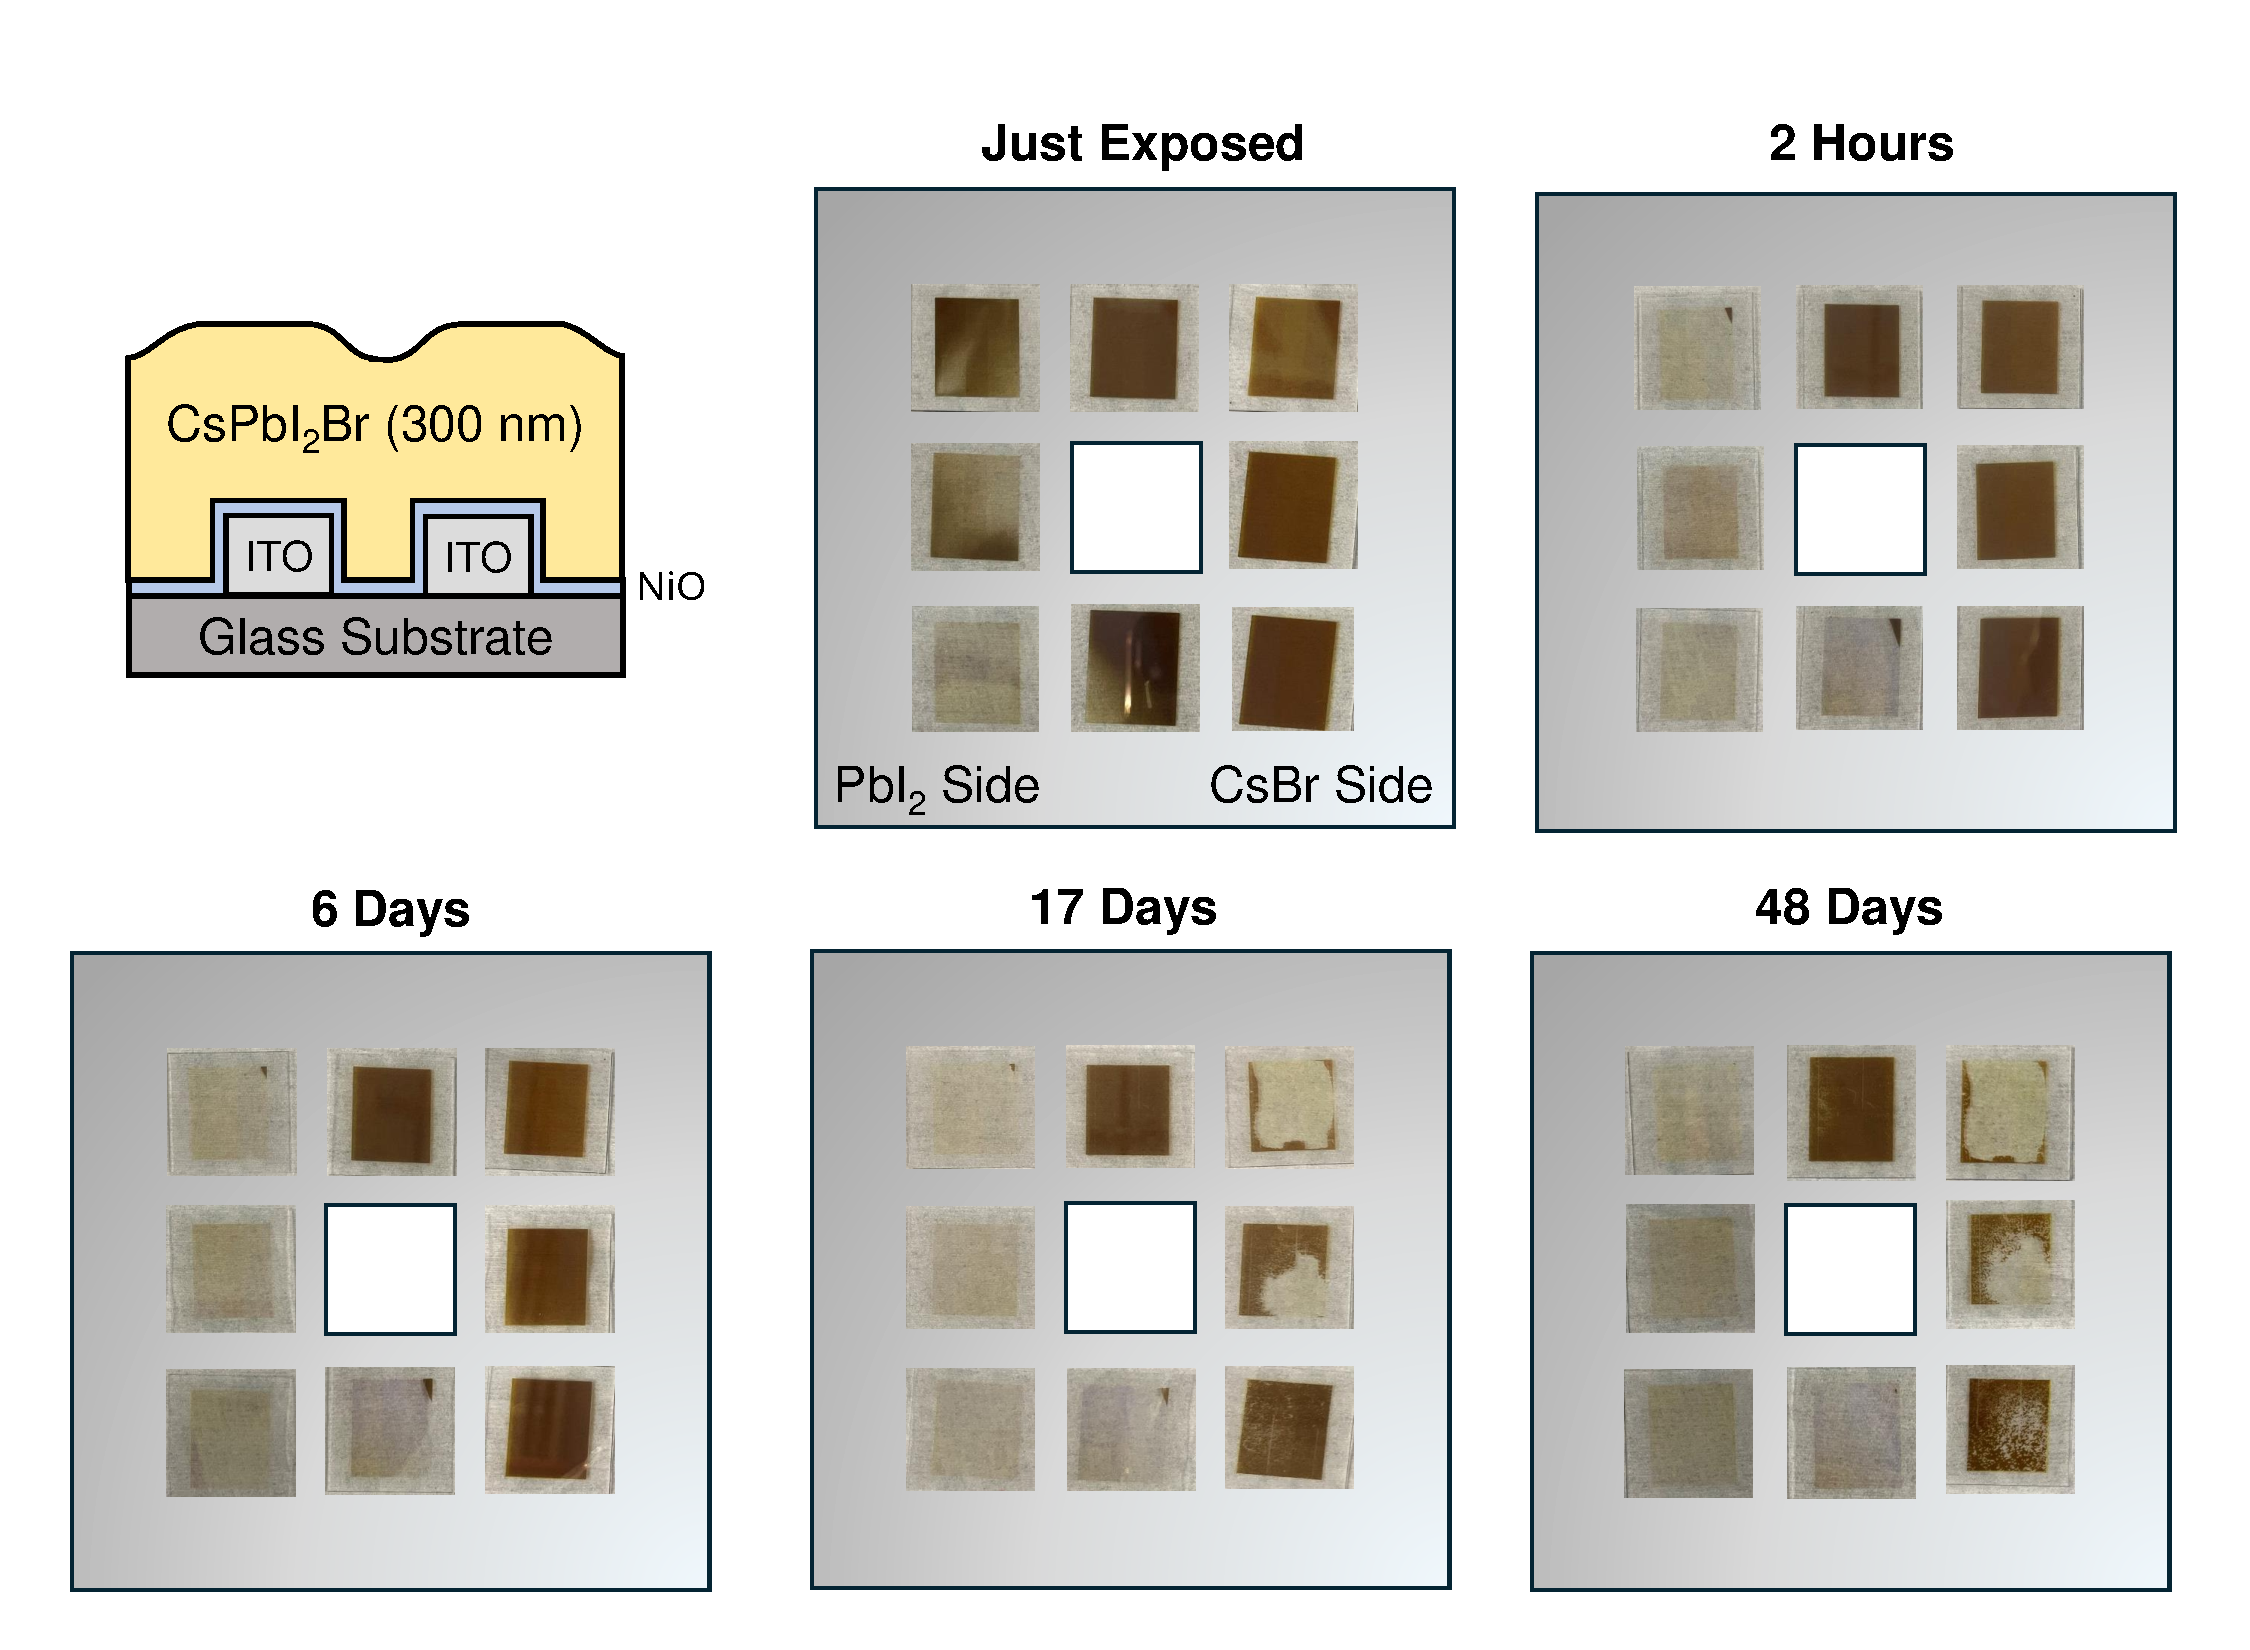
\includegraphics[width=\textwidth]{chapters/appendixB/images/Stability_No_Rotation_275_on_nio_repeated.pdf} % Replace with your image file
             
    \end{subfigure}

\caption[Assessment of the ambient stability repeatability of 300-nm-thick \ch{CsPbI_2Br} thin films deposited via combinatorial co-evaporation on glass/ITO substrates coated with a 15 nm NiO\textsubscript{x} layer.]{Assessment of the ambient stability repeatability of 300-nm-thick \ch{CsPbI_2Br} thin films deposited via combinatorial co-evaporation on glass/ITO substrates coated with a 15 nm NiO\textsubscript{x} layer. This set of samples originates from a repetition of the deposition whose results were presented in Figure~\ref{fig:stability:no_rotation:300nm_ito_nio}.}
\label{fig:appendix:stability_on_NiO_v2}
\end{figure}

%%%%%%%%%%%%%%%%%%%%%%%%%%%%%%%%%%%%%%%%%%%%%%%%%%
% Keep the following \cleardoublepage at the end of this file, 
% otherwise \includeonly includes empty pages.
\cleardoublepage

% vim: tw=70 nocindent expandtab foldmethod=marker foldmarker={{{}{,}{}}}
